\documentclass{article}
\usepackage{amsmath}
\usepackage{amssymb}
\usepackage[svgnames]{xcolor}
\usepackage{graphicx}
\usepackage{enumitem}
\usepackage{multicol}
\usepackage{graphicx}
\usepackage{color}


\begin{document}
\section{Sum-product Algorithm}
\begin{figure}[htb!]
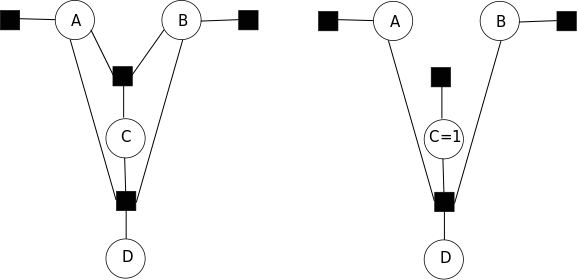
\includegraphics[width = \textwidth]{ex01.png}
\end{figure}

The graph is now in tree structure, acyclic.
\begin{table}[htb]
\caption{$f_A$}
\centering
  \begin{tabular}{ | c | c | c | c | c | c | c | c |}
    \hline
    A & B & C & D & $f_A$ & $f_B$ & $f_C$ & $f_D$ \\ \hline
    1 & 1 & 1 & 1 & 1 & 1 & 1 & 1\\\hline
    0 & 0 & 1 & 0 & 0 & 0 & 0 & 1\\\hline
    1 & 0 & 1 & 0 & 1 & 0 & 1 & 1\\\hline
    0 & 1 & 1 & 0 & 0 & 1 & 1 & 0\\\hline
	0 & 0 & 1 & 1 & 0 & 0 & 0 & 0\\\hline
	1 & 1 & 1 & 0 & 0 & 0 & 0 & 0\\\hline
	1 & 0 & 1 & 1 & 0 & 0 & 0 & 0\\\hline
	0 & 1 & 1 & 1 & 0 & 0 & 0 & 0\\\hline

  \end{tabular}
\end{table}

\section{Project Orientation}
\begin{enumerate}
\item \textbf{SketchNet: Sketch Classification with Web Images (Zhang et al.)} They use a deep neural network consisting of three sub networks with distinct tasks (feature extraction of real images, feature extraction of sketch images, detection of common structures in both image categories)  to classify sketches. Reason for picking this paper: They have an interesting approach to find common structures in sketch and real images: they give pairs of sketch and real images as training data, where they picked as negative instances something like the support vectors (the 5-nn of the 5 most likely false positive predicted classes for each sketch). Giving the hardest examples as negative training data supposedly leads to a steeper learning curve. Also the approach of finding similar structure in images of different modalities (real/sketch) could be applied to other areas e.g. medical imaging where images of different modalities (CT, MRI, angiography etc) are matched.
\item \textbf{Object Skeleton Extraction in Natural Images by Fusing Scale-associated Deep
Side Outputs (Shen et al.)} Here a fully convolutional network for skeleton extraction is introduced. They approach the problem as a multi-class problem instead of a binary (skeleton = 1, no skeleton = 0) approach, by labeling each skeleton pixel with the minimal disk size where the feature can still be extracted. The convolutional layers equal filters of increasing receptive field size and they add a supervision stage at each convolutional layer comparing the filter output to the scale related ground truth. Reason to pick this paper: we assume that adding supervision to several stages of a convolutional network as done in this paper could be advantageous to several other problems. Also it would be interesting to know how this model performs on 3D data.
\item \textbf{Where are they looking? (Recasens et al.)}
\end{enumerate}
\end{document}